\renewcommand{\theequation}{\theenumi}
\begin{enumerate}[label=\thesection.\arabic*.,ref=\thesection.\theenumi]
\numberwithin{equation}{enumi}

\item Vertices of the quadrilateral are,
\begin{align}
\vec{A}=\myvec{-4\\5}
\vec{B}=\myvec{0\\7}
\vec{C}=\myvec{5\\-5}
\vec{D}=\myvec{-4\\-2}
\end{align}
Quadrilateral ABCD is drawn by joining its vertices $\vec{A}$ and $\vec{B}$,$\vec{B}$ and $\vec{C}$, $\vec{C}$ and $\vec{D}$, $\vec{D}$ and $\vec{A}$.
 The  following Python code generates Fig. \ref{fig:quad_py}
%
\begin{lstlisting}
codes/quad/quad.py
\end{lstlisting}
\begin{figure}[!ht]
\centering
\includegraphics[width=\columnwidth]{./codes/quad/pyfigs/quad.eps}
\caption{Quadrilateral ABCD}
\label{fig:quad_py}
\end{figure}

\item From Figure \ref{fig:quad_py} Area of the Quadrilateral ABCD can be given as
\begin{align}
Ar\brak{\triangle ABC} + Ar\brak{\triangle BCD}
\\
\frac{1}{2} \norm{\brak{\vec{A}-\vec{B}}\times \brak{\vec{A}-\vec{D}}} + \frac{1}{2} \norm{{\brak{\vec{C}-\vec{B}}} \times{\brak{\vec{C}-\vec{D}}}}
\\
=60.5 sq.units
\end{align}
\end{enumerate}
